%%%%%%%%%%%%%%%%%%%%%%%%%%%%%%%%%%%%%%%%%%%%%%
%% Compile: XeLaTeX BibTeX XeLaTeX XeLaTeX
%% Slides: Stefan Müller
%% Course: GK Linguistik
%%%%%%%%%%%%%%%%%%%%%%%%%%%%%%%%%%%%%%%%%%%%%%

\documentclass[a4paper,10pt, bibtotoc]{beamer}
%\documentclass[10pt,handout]{beamer}

%%%%%%%%%%%%%%%%%%%%%%%%
%%     PACKAGES & COMMANDS
%%%%%%%%%%%%%%%%%%%%%%%%

%%%%%%%%%%%%%%%%%%%%%%%%
%%     PACKAGES       %%
%%%%%%%%%%%%%%%%%%%%%%%%



%\usepackage[utf8]{inputenc}
%\usepackage[vietnamese, english,ngerman]{babel}   % seems incompatible with german.sty
%\usepackage[T3,T1]{fontenc} breaks xelatex
\usepackage{lmodern}

\usepackage{amsmath}
\usepackage{amsfonts}
\usepackage{amssymb}
%% MnSymbol: Mathematische Klammern und Symbole (Inkompatibel mit ams-Packages!)
%% Bedeutungs- und Graphemklammern: $\lsem$ Tisch $\rsem$ $\langle TEXT \rangle$ $\llangle$ TEXT $\rrangle$ 
\usepackage{MnSymbol}
%% ulem: Strike out
\usepackage[normalem]{ulem}  

%% Special Spaces (s. Commands)
\usepackage{xspace}				
\usepackage{setspace}
%	\onehalfspacing

%% mdwlist: Special lists
\usepackage{mdwlist}	

\usepackage[noenc,safe]{tipa}

% maybe define \textipa to use \originalTeX to avoid problems with `"'.
%
%	\ex \textipa{\originalTeX [pa.pa."g\t{aI}]}

%

\usepackage{etex}		%For Forest bug

%
%\usepackage{jambox}
%


%\usepackage{forest-v105}
%\usepackage{modified-langsci-forest-setup}

\usepackage{xeCJK}
\setCJKmainfont{SimSun}


%\usepackage{natbib}
%\setcitestyle{notesep={:~}}




% for toggles
\usepackage{etex}



% Fraktur!
\usepackage{yfonts}

\usepackage{url}

% für UDOP
\usepackage{adjustbox}


%% huberlin: Style sheet
%\usepackage{huberlin}
\usepackage{hu-beamer-includes-pdflatex}
\huberlinlogon{0.86cm}


%% Last Packages
%\usepackage{hyperref}	%URLs
%\usepackage{gb4e}		%Linguistic examples

% sorry this was incompatible with gb4e and had to go.
%\usepackage{linguex-cgloss}	%Linguistic examples (patched version that works with jambox

\usepackage{multirow}  %Mehrere Zeilen in einer Tabelle
%\usepackage{array}
\usepackage{marginnote}	%Notizen




%%%%%%%%%%%%%%%%%%%%%%%%%%%%%%%%%%%%%%%%%%%%%%%%%%%%
%%%          Commands                            %%%
%%%%%%%%%%%%%%%%%%%%%%%%%%%%%%%%%%%%%%%%%%%%%%%%%%%%

%%%%%%%%%%%%%%%%%%%%%%%%%%%%%%%%
% German quotation marks:
\newcommand{\gqq}[1]{\glqq{}#1\grqq{}}		%double
\newcommand{\gq}[1]{\glq{}#1\grq{}}			%simple


%%%%%%%%%%%%%%%%%%%%%%%%%%%%%%%%
% Abbreviations in German
% package needed: xspace
% Short space in German abbreviations: \,	
\newcommand{\idR}{\mbox{i.\,d.\,R.}\xspace}
\newcommand{\su}{\mbox{s.\,u.}\xspace}
%\newcommand{\ua}{\mbox{u.\,a.}\xspace}       % in abbrev
%\newcommand{\zB}{\mbox{z.\,B.}\xspace}       % in abbrev
%\newcommand{\s}{s.~}
%not possibel: \dh --> d.\,h.


%%%%%%%%%%%%%%%%%%%%%%%%%%%%%%%%
%Abbreviations in English
\newcommand{\ao}{a.o.\ }	% among others
\newcommand{\cf}[1]{(cf.~#1)}	% confer = compare
\renewcommand{\ia}{i.a.}	% inter alia = among others
\newcommand{\ie}{i.e.~}	% id est = that is
\newcommand{\fe}{e.g.~}	% exempli gratia = for example
%not possible: \eg --> e.g.~
\newcommand{\vs}{vs.\ }	% versus
\newcommand{\wrt}{w.r.t.\ }	% with respect to


%%%%%%%%%%%%%%%%%%%%%%%%%%%%%%%%
% Dash:
\newcommand{\gs}[1]{--\,#1\,--}


%%%%%%%%%%%%%%%%%%%%%%%%%%%%%%%%
% Rightarrow with and without space
\def\ra{\ensuremath\rightarrow}			%without space
\def\ras{\ensuremath\rightarrow\ }		%with space


%%%%%%%%%%%%%%%%%%%%%%%%%%%%%%%%
%% X-bar notation

%% Notation with primes (not emphasized): \xbar{X}
\newcommand{\MyPxbar}[1]{#1$^{\prime}$}
\newcommand{\xxbar}[1]{#1$^{\prime\prime}$}
\newcommand{\xxxbar}[1]{#1$^{\prime\prime\prime}$}

%% Notation with primes (emphasized): \exbar{X}
\newcommand{\exbar}[1]{\emph{#1}$^{\prime}$}
\newcommand{\exxbar}[1]{\emph{#1}$^{\prime\prime}$}
\newcommand{\exxxbar}[1]{\emph{#1}$^{\prime\prime\prime}$}

% Notation with zero and max (not emphasized): \xbar{X}
\newcommand{\zerobar}[1]{#1$^{0}$}
\newcommand{\maxbar}[1]{#1$^{\textsc{max}}$}

% Notation with zero and max (emphasized): \xbar{X}
\newcommand{\ezerobar}[1]{\emph{#1}$^{0}$}
\newcommand{\emaxbar}[1]{\emph{#1}$^{\textsc{max}}$}

%% Notation with bars (already implemented in gb4e):
% \obar{X}, \ibar{X}, \iibar{X}, \mbar{X} %Problems with \mbar!
%
%% Without gb4e:
\newcommand{\overbar}[1]{\mkern 1.5mu\overline{\mkern-1.5mu#1\mkern-1.5mu}\mkern 1.5mu}
%
%% OR:
\newcommand{\MyPibar}[1]{$\overline{\textrm{#1}}$}
\newcommand{\MyPiibar}[1]{$\overline{\overline{\textrm{#1}}}$}
%% (emphasized):
\newcommand{\eibar}[1]{$\overline{#1}$}
\newcommand{\eiibar}[1]{\overline{$\overline{#1}}$}

%%%%%%%%%%%%%%%%%%%%%%%%%%%%%%%%
%% Subscript & Superscript: no italics
\newcommand{\MyPdown}[1]{$_{\textrm{#1}}$}
\newcommand{\MyPup}[1]{$^{\textrm{#1}}$}


%%%%%%%%%%%%%%%%%%%%%%%%%%%%%%%%
% Objekt language marking:
%\newcommand{\obj}[1]{\glqq{}#1\grqq{}}	%German double quotes
%\newcommand{\obj}[1]{``#1''}			%English double quotes
\newcommand{\MyPobj}[1]{\emph{#1}}		%Emphasising


%%%%%%%%%%%%%%%%%%%%%%%%%%%%%%%%
%% Semantic types (<e,t>), features, variables and graphemes in angled brackets 

%%% types and variables, in math mode: angled brackets + italics + no space
%\newcommand{\type}[1]{$<#1>$}

%%% OR more correctly: 
%%% types and variables, in math mode: chevrons! + italics + no space
\newcommand{\MyPtype}[1]{$\langle #1 \rangle$}

%%% features and graphemes, in math mode: chevrons! + italics + no space
\newcommand{\abe}[1]{$\langle #1 \rangle$}


%%% features and graphemes, in math mode: chevrons! + no italics + space
\newcommand{\ab}[1]{$\langle$#1$\rangle$}  %%same as \abu  
\newcommand{\abu}[1]{$\langle$#1$\rangle$} %%Umlaute

%%% Notizen
\renewcommand{\marginfont}{\singlespacing}
\renewcommand{\marginfont}{\footnotesize}
\renewcommand{\marginfont}{\color{black}}

\newcommand{\myp}[1]{%
	\marginnote{%
		\begin{spacing}{1}
			\vspace{-\baselineskip}%
			\color{red}\footnotesize#1
		\end{spacing}
	}
}
%%%%%%%%%%%%%%%%%%%%%%%%%%%%%%%%
%% Outputbox
\newcommand{\outputbox}[1]{\noindent\fbox{\parbox[t][][t]{0.98\linewidth}{#1}}\vspace{0.5em}}

%%%%%%%%%%%%%%%%%%%%%%%%%%%%%%%%
%% (Syntactic) Trees
% package needed: forest
%
%% Setting for simple trees
\forestset{
	MyP edges/.style={for tree={parent anchor=south, child anchor=north}}
}

%% this is taken from langsci-setup file
%% Setting for complex trees
%% \forestset{
%% 	sn edges/.style={for tree={parent anchor=south, child anchor=north,align=center}}, 
%% background tree/.style={for tree={text opacity=0.2,draw opacity=0.2,edge={draw opacity=0.2}}}
%% }

\newcommand\HideWd[1]{%
	\makebox[0pt]{#1}%
}


%%%%%%%%%%%%%%%%%%%%%%%%%%%%%%%%%%%%%%%%%%%%%%%%%%%%
%%%          Useful commands                     %%%
%%%%%%%%%%%%%%%%%%%%%%%%%%%%%%%%%%%%%%%%%%%%%%%%%%%%

%%%%%%%%%%%%%%%%%%%%%
%% FOR ITEMS:
%\begin{itemize}
%  \item<2-> from point 2
%  \item<3-> from point 3 
%  \item<4-> from point 4 
%\end{itemize}
%
% or: \onslide<2->
% or: \pause

%%%%%%%%%%%%%%%%%%%%%
%% VERTICAL SPACE:
% \vspace{.5cm}
% \vfill

%%%%%%%%%%%%%%%%%%%%%
% RED MARKING OF TEXT:
%\alert{bis spätestens Mittwoch, 18 Uhr}

%%%%%%%%%%%%%%%%%%%%%
%% RESCALE BIG TABLES:
%\scalebox{0.8}{
%For Big Tables
%}

%%%%%%%%%%%%%%%%%%%%%
%% BLOCKS:
%\begin{alertblock}{Title}
%Text
%\end{alertblock}
%
%\begin{block}{Title}
%Text
%\end{block}
%
%\begin{exampleblock}{Title}
%Text
%\end{exampleblock}


\newtoggle{uebung}
\newtoggle{loesung}
\newtoggle{toc}

% The toc is not needed on Handouts. Safe trees.
\mode<handout>{
\togglefalse{toc}
}

\newtoggle{hpsgvorlesung}\togglefalse{hpsgvorlesung}
\newtoggle{syntaxvorlesungen}\togglefalse{syntaxvorlesungen}

%\includecomment{psgbegriffe}
%\excludecomment{konstituentenprobleme}
%\includecomment{konstituentenprobleme-hinweis}

\newtoggle{konstituentenprobleme}\togglefalse{konstituentenprobleme}
\newtoggle{konstituentenprobleme-hinweis}\toggletrue{konstituentenprobleme-hinweis}

%\includecomment{einfsprachwiss-include}
%\excludecomment{einfsprachwiss-exclude}
\newtoggle{einfsprachwiss-include}\toggletrue{einfsprachwiss-include}
\newtoggle{einfsprachwiss-exclude}\togglefalse{einfsprachwiss-exclude}

\newtoggle{psgbegriffe}\toggletrue{psgbegriffe}

\newtoggle{gb-intro}\togglefalse{gb-intro}



%%%%%%%%%%%%%%%%%%%%%%%%%%%%%%%%%%%%%%%%%%%%%%%%%%%%
%%%             Preamble's End                   
%%%%%%%%%%%%%%%%%%%%%%%%%%%%%%%%%%%%%%%%%%%%%%%%%%%% 

\begin{document}
	
	
%%%% ue-loesung
%%%% true: Übung & Lösungen (slides) / false: nur Übung (handout)
\toggletrue{ue-loesung}

%%%% ha-loesung
%%%% true: Hausaufgabe & Lösungen (slides) / false: nur Hausaufgabe (handout)
\toggletrue{ha-loesung}

%%%% toc
%%%% true: TOC am Anfang von Slides / false: keine TOC am Anfang von Slides
\toggletrue{toc}

%%%% sectoc
%%%% true: TOC für Sections / false: keine TOC für Sections (StM handout)
\toggletrue{sectoc}

%%%% gliederung
%%%% true: Gliederung für Sections / false: keine Gliederung für Sections
%	\toggletrue{gliederung}



\author[St.Mü.]{
	{Stefan Müller}
%	\\
%	{\footnotesize \url{http://www.linguistik.hu-berlin.de/staff/amyp}\\
%	\href{mailto:mapriema@hu-berlin.de}{mapriema@hu-berlin.de}}
}

\institute{Institut für deutsche Sprache und Linguistik}


%% -*- coding:utf-8 -*-

\title{Grundkurs Linguistik}

\subtitle{Morphologie}


\huberlintitlepage[22pt]

\section{Morphologie}

\author{Stefan Müller (Anke Lüdeling)}

\frame{
\frametitle{Morphologie: Material}


\citew[Kapitel~7 und 8]{Luedeling2009a}, \citew{Haspelmath2002a}




}


\frame{
\frametitle{Morphologie}


\begin{itemize}
\item Die Morphologie beschäftigt sich mit dem Aufbau komplexer Wörter.
\ea
des Brunnenkressesüppchens \citep{Luedeling2009a}
\z

Das Wort in (\mex{0}) kann man wie folgt zerteilen (((Brunnen-kresse)-süpp)-chen)-s =

Genitivform (\suffix{s}) einer kleinen (\suffix{chen}) Suppe (\emph{süpp}) mit Brunnenkresse.
\pause

\item Es gibt morphologische Bestandteile, die frei (alleine) vorkommen können (\emph{Brunnen}, \emph{Kresse},
  \emph{Suppe})
\pause
\item Es gibt morphologische Bestandteile, die nicht frei vorkommen können (\suffix{chen},
  \suffix{s}).

\pause
\item Manche Bestandteile verändern in bestimmten Umgebungen ihre Form (\emph{Suppe} vor
  \suffix{chen} $\to$ \emph{süpp}).

\pause
\item Struktur spiegelt die Bedeutung eines komplexen Ausdrucks wider.
\end{itemize}



}

\frame{
\frametitle{Wortbildung und Flexion}


Teile des Wortes machen die Bedeutung aus und könnten einen Lexikoneintrag bilden:
\emph{Brunnenkressesüppchen}.

Diese Grundform oder auch Zitierform nennt man \blaubf{Lemma}.

Die anderen Teile bestimmen die grammatischen Eigenschaften:\\
\suffix{s} = Genitiv.

Der Teil der Morphologie, der sich mit der Bildung von Lemmata beschäftigt, heißt
\blaubf{Worbildungslehre}.

Die grammatischen Formen werden in der \blaubf{Flexionsmorphologie} behandelt.


}


\subsection{Der Wortbegriff}



\frame{
\frametitle{Der Wortbegriff}

Obwohl Wörter eine zentrale Rolle in der Grammatikforschung spielen,\\
wird immer noch kontrovers diskutiert, was ein Wort ist.

Kriterien:
\begin{itemize}
\item orthographisch-graphemische
\item phonetisch-phonologische
\item morphologische
\item lexikalisch-semantische
\item syntaktische
\end{itemize}

Siehe \citew{Bussmann2002a}.

}

\subsubsection{Die orthographisch-graphemische Ebene}

\frame{
\frametitle{Die orthographisch-graphemische Ebene}

Wörter werden durch Leerzeichen voneinander getrennt.

\pause
Problem 1: Komposita im Englischen:
\eal
\ex summer school
\ex Sommerschule
\zl

\pause

Städtenamen im Deutschen:
\eal
\ex New York
\ex Berlin
\zl

}

%\begin{CJK*}{UTF8}{code2k}% Aus irgendwelchen Gründen zeigt gbsn die Punkte nicht an.


\frame{
\frametitle{Wörter sind durch Leerzeichen abgetrennt}

Problem 2: Chinesisch


%\begin{CJK*}{UTF8}{gbsn} % ist jetzt gefixt (SuSE 11.1)
近年来,``应用语言学''作为语言学的一个分支,在国内外都得到了较大的发展,但对于``什么是应用语言学'',
``应用语言学包括哪些研究领域'' 等最基本的问题,学者们却始终没有一个统一的看法。对于一门发展中的、涉及内容广泛的学科而言这是正常的,但长期下去,又会对学科的发展产生不利影响。
%\end{CJK*}

Chinesische Wörter können aus einem oder mehreren Symbolen bestehen.\\
Texte werden von oben nach unten geschrieben.\\
Auf Computern von links nach rechts.\\
Es gibt keine Leerzeichen zwischen Wörtern.

}



\frame{
\frametitle{Wörter sind durch Leerzeichen abgetrennt}

\begin{itemize}
\item Problem 3: Sprachen ohne Schriftsystem

Es gibt Sprachen, für die noch kein Schriftsystem erarbeitet wurde.

\pause

\item Problem 4: die Rechtschreibreform

Hat sich im Deutschen der Wortstatus bestimmter Buchstabenfolgen in den letzten Jahren mehrmals geändert?

\pause

Nein! Die Schriftsprache ist sekundär. 

\pause
Im besten Fall wurde das Schriftsystem von fähigen Linguisten entwickelt.
\pause

Im schlechtesten Fall spiegelt es verschiedene Stufen der historischen Entwicklung einer Sprache und diverse
Kompromisse von normierenden Institutionen wider.
\end{itemize}

}


\subsubsection{Die phonetisch-phonologische Ebene}

\frame{
\frametitle{Die phonetisch-phonologische Ebene}

Wörter sind kleinste, durch Wortakzent und Grenzsignale wie Pause, Knacklaut u.\,a.\ theoretisch
isolierbare Lautsegmente.


Das funktioniert nicht immer, da wir ohne "`Punkt und Komma"' reden.

In manchen Sprachen gibt es Phänomene wie Vokalharmonie,\\
die einen Rückschluss auf das Wortende erlauben.

}

\subsubsection{Die morphologische Ebene}

\frame{
\frametitle{Die morphologische Ebene}

Wörter sind als Grundeinheiten von grammatischen Paradigmen wie Flexion gekennzeichnet und zu
unterscheiden von den morphologisch charakterisierten Wortformen (\emph{schreiben} vs.\
\emph{schreibst}, \emph{schrieb}, \emph{geschrieben}).

\pause

Problem: Es gibt unflektierbare Wörter.


}


\subsubsection{Die lexikalisch-semantische Ebene}

\frame{
\frametitle{Die lexikalisch-semantische Ebene}

Wörter sind die kleinsten, relativ selbständigen Träger von Bedeutung,\\
die im Lexikon kodifiziert sind.

\pause
Problem: Unikale Elemente
\eal
\ex \blaubf{klipp} und klar
\ex auf \blaubf{Anhieb}
\zl

%\pause
%Außerdem: War das nicht die Definition für Morphem?

}


\subsubsection{Die syntaktische Ebene}

\frame{
\frametitle{Die syntaktische Ebene}

Wörter sind die kleinsten verschiebbaren und ersetzbaren Einheiten des Satzes.
\pause

Ist \emph{anfangen} ein Wort oder zwei?
\eal
\ex weil nächste Woche die Schule anfängt
\ex Nächste Woche fängt die Schule an.
\zl


}


\subsubsection{Ein Ausweg?}

\frame{
\frametitle{Ein Ausweg?}


Ein Ausweg besteht darin, das Wort \emph{Wort} an den Stellen nicht mehr zu verwenden, an denen
Mißverständnisse aufkommen könnten.

Statt dessen \blaubf{Morphem}, \blaubf{Lexem} und \blaubf{Wortform}.


}

\subsubsection{Lexem}

\frame{
\frametitle{Lexem}


\blaubf{Lexeme} sind die lexikalischen Einheiten der Sprache.

Lexeme können (je nach Wortart) ein Paradigma bilden:

\eal
\ex lach-: lache, lachst, lacht, lachen, lacht, lachen, lachte, \ldots
\ex Mann-: \begin{tabular}[t]{@{}l@{~}l@{~}l@{~}l@{}}
           Mann, & Mannes, & Mann(e), & Mann\\
           Männer, & Männer, & Männern, & Männer\\
           \end{tabular}
\zl

\pause

Ein \blaubf{Lemma} ist eine (möglichst sinnvolle) Bezeichnung für ein Lexem:\\
\emph{lachen} für (\mex{0}a), \dash Infinitivform bei Verben\\
\emph{Mann} für (\mex{0}b), \dash Nominativ Singular bei Nomen

\pause

Komplexe Einheiten wie (\mex{1})  werden als \blaubf{Mehrwortlexeme} bezeichnet.

\eal
\ex klipp und klar
\ex ins Gras beiß-
\zl


}

\subsubsection{Wortform}

\frame{
\frametitle{Wortform}

Die verschiedenen Formen, die zum Paradigma eines Lexems gehören, werden \blaubf{Wortformen} genannt.

}



\subsubsection{Morphem}

\frame{
\frametitle{Morphem (klassische Definition)}


Ein \blaubf{Morphem} ist die kleinste, nicht mehr reduzierbare bedeutungstragende sprachliche Einheit.

Lexeme sind lexikalische Morpheme im Gegensatz zu (nur) grammatikalischen Morphemen, wie \zb Flexionsmorphemen.



}


\frame{
\frametitle{Morphem (revidierte Definition)}


 Ein \blaubf{Morphem} ist die kleinste, in ihren verschiedenen Vorkommen
 als formal einheitlich identifizierbare Folge von Segmenten, der
 (wenigstens) eine als einheitlich identifizierbare
 außerphonologische Eigenschaft zugeordnet ist. (Wurzel 1984:38)

\pause

 Bedeutung ist eine außerphonologische Eigenschaft

\begin{tabular}{@{}ll@{}}
  Pluralbildung:         & \suffix{er}\\
  `wie ein':             & \suffix{lich}\\
\end{tabular}

\pause

 Andere grammatische Merkmale werden ebenfalls morphologisch
 ausgedrückt:

\begin{tabular}{@{}ll@{}}
  Infinitivbildung:     &  \suffix{en}
\end{tabular}

}

\subsubsection{Allomorphe}

\frame{
\frametitle{Morpheme und Allomorphe}


Mitunter gibt es zu einem Morphem mehrere Morphe:

\begin{tabular}{lllll}
Morphem & Morph & Morph & Morph & Morph\\
{\sc Tee} & $<$tee$>$\\
{\sc suppe} & $<$suppe$>$ & $<$süpp$>$ \\
           &        & wie in \emph{Süpp-chen}\\
{\sc Brot} & $<$brot$>$ & $<$bröt$>$\\
           &        & wie in \emph{Bröt-chen}\\
-{\sc chen} & $<$chen$>$\\
{\sc Plural} & $<$e$>$  & $<$en$>$ & $<$er$>$ & \ldots\\ 

\end{tabular}

Diese werden auch \blaubf{Allomorphe} genannt.

Man kann so vom Plural-Morphem reden,\\
obwohl es viele verschiedene Realisierungsmöglichkeiten gibt.

}


\subsubsection{Suppletion}

\frame{
\frametitle{Suppletion}

\eal
\ex schön -- schöner -- am schönsten
\ex gut -- besser -- am besten
\zl

Sind \emph{gut}, \emph{bess} und \emph{be} Allomorphe desselben Morphems?

\pause

\emph{gut}, \emph{besser}, \emph{am besten} und \emph{sein}, \emph{bin}, \emph{ist}, \emph{war} sind
historisch zu  erklären:\\
Zwei oder mehrere Flexionsparadigmen sind zusammengefallen.

\pause

Solche Muster sind als Ausnahmen zu behandeln.


}

\subsubsection{Freie und gebundene Morpheme, Affixe}

\frame{
\frametitle{Freie und gebundene Morpheme, Affixe}

Morpheme, die durch mindestens ein Morph realisiert werden,\\
das auch alleine vorkommen kann, nennt man \blaubf{freie Morpheme}.

\pause
Morpheme, die nur durch Morphe realisiert werden, die nicht alleine vorkommen können, nennt man
\blaubf{gebundene Morpheme} oder \blaubf{Affixe}.

Beispiel: -{\sc chen}.


}


\subsubsection{Affixe}

\frame{
\frametitle{Affixe}

\begin{itemize}
\item Affixe, die vor anderen Morphemen stehen, heißen \blaubf{Präfixe}.

Beispiel: {\sc ver}-

\pause
\item Affixe, die nach anderen Morphemen stehen, heißen \blaubf{Suffixe}.

Beispiel: -{\sc chen}

\pause

\item Affixe, die andere Morpheme einschließen, heißen \blaubf{Zirkumfixe}.

Beispiel: {\sc ge}- -{\sc e} in \emph{Gerenne}.

\end{itemize}


}


\subsubsection{Stamm}

%\author{Stefan Müller}
\frame{
\frametitle{Stamm}

% Todo: Stimmt nicht
%Für jedes Morphem gibt es ein Allomorph,\\
%das in der Wortbildung hauptsächlich verwendet wird.


Morpheme (\emph{schön}) oder Morphemkonstruktionen (\emph{un-schön}, \emph{Schön-heit}),\\
an die Flexionsendungen treten können, werden \blaubf{Stamm} genannt.


Nomina: identisch mit dem Nominativ Singular: \emph{Baum}, \emph{Katze}, \emph{Kind}

Adjektive: prädikative Form: \emph{blau}, \emph{schlau}, \emph{genau}

Verben: Infinitivform ohne Infinitivendung: \emph{lauf}, \emph{sing}

\pause

Stämme, die nicht zerlegt werden können, heißen \blaubf{Wurzel}.


}



\subsubsection{Simplizia und komplexe Lexeme}


\frame{
\frametitle{Simplizia und komplexe Lexeme}

\begin{itemize}
\item Lexeme, die nur aus einem Allomorph eines freien Morphems bestehen, nennt man
  \blaubf{Simplizia}.

Diese sind für die Morphologie uninteressant,\\
da sie nicht zerlegt werden können.

\pause
\item Komplexe Lexeme werden durch Anwendung eines Prozesses/einer Regel auf ein Grundmorphem
  erzeugt.

\pause
\item Einfachster Prozess ist Aneinanderhängen (Konkatenation).

\pause
\item Im Deutschen zwei konkatenative Wortbildungsprozesse:\\
      Komposition und Derivation
\end{itemize}

}


\subsection{Wortbildung}

\subsubsection{Komposition}


% taz, berlin 2.5.2011: Zwangsräumungsklageunterwerfungsklausel 

\frame{
\frametitle{Wortbildung: Komposition}

\begin{itemize}
% Todo: Stimmt nicht: Verben, stimmt doch, Imperativform von Verben
\item Komposition = Konkatenation von Allomorphen freier Morpheme (\emph{wein+rot})
%\item Komposition = Konkatenation von Allomorphen von Lexemen (\emph{wein+rot})
\pause
\item Nominalkomposition
\begin{tabular}{lll}
Muster & Beispiele & Regel \\
Nomen+Nomen & Erbsensuppe, & N $\to$ N N\\
            & Hundefutter, Gasherd &\\
%
Adjektiv+Nomen & Rotwein, Grünkohl & N$_1$ $\to$ Adj N$_2$\\
               & Hartweizen &\\
%
Verb+Nomen & Esslöffel, & N$_1$ $\to$ V N$_2$\\
           & Rührschüssel &\\
           & Kehrblech &\\
Adverb+Nomen & Beinahekatastrophe & N$_1$ $\to$ Adv N$_2$\\
             & Soforthilfe&\\
\end{tabular}

\end{itemize}

}

\frame{
\frametitle{Strukturbaum zur Visualisierung der Regeln}

\vfill

\hfill
\begin{forest}
sm edges
[N
  [N [Gas]]
  [N [herd]]]
\end{forest}
\hfill\hfill\mbox{}


\vfill

}


\subsubsubsection{Köpfe, Rekursion, Fugen}

%\subsubsubsection{Morphologische Köpfe}

\frame{
\frametitle{Morphologische Köpfe}

\begin{itemize}
\item In deutschen Komposita wird die Wortart immer vom rechten Element bestimmt:
\eal
\ex Haustür    
\ex affengeil
\zl
\pause
\item Bei Nomina wird auch das Genus vom rechten Element übernommen:
\eal
\ex das Haus
\ex die Tür
\ex die Haustür
\zl
\pause
\item Die meisten Wortbildungsprodukte haben einen Kopf, \\
\dash ein Element, das die Eigenschaften des komplexen Wortes bestimmt.
\pause
\item Meistens auch die Grundbedeutung (\emph{Wildkatze}, \emph{Küchentisch})
\pause
\item Stellung des Kopfes ist sprachspezifisch.

\end{itemize}

}

%\subsubsubsection{Rekursion}
\frame{
\frametitle{Rekursion}

\begin{itemize}
\item Bildung von Komposita kann mit nominalen Bestandteilen sehr komplex werden:
\ea
Gasherdverkäuferschulungszentrumseinrichtungsbudget
%Rindfleischettikettierungsüberwachungsaufgabenübertragungsgesetz
% http://www.youtube.com/watch?v=P455AFT4cWw
\z
\pause
\item Das wird durch die angegebene Regel erfasst:
\ea
N $\to$ N N
\z
Das, was die Regel erzeugt, kann selbst wieder in die rechte Regelseite eingesetzt werden. 

Solche Regeln werden \blaubf{rekursiv} genannt.
\end{itemize}




}

\frame{
\frametitle{Keine Rekursion}

\begin{itemize}
\item Mit Adjektiven als Erstglied ist keine Rekursion möglich:
\eal
\ex[*]{
Samtigrotwein
}
\ex[*]{
Weißmagerquark
}
\ex[*]{
Feuchtgrünfutter
}
\zl
Das wird dadurch erfasst, dass auf der linken Regelseite ein anderes Symbol verwendet wird:
\ea
N$_1$ $\to$ Adj N$_2$
\z

(Allerdings: Frühneuhochdeutsch, Billigrotwein)

\pause
\item In die NN-Regel können N$_1$ und N$_2$ eingesetzt werden. 
\ea
N $\to$ N N
\z
N steht für beides.

\end{itemize}




}

%\subsubsubsection{Fugen}

\frame{
\frametitle{Fugen}

\begin{itemize}
\item Welchen Status hat das markierte Material in (\mex{1})?
\eal
\ex Hund\blaubf{e}futter
\ex Erbse\blaubf{n}suppe
\zl
\pause
\item Ist es die Pluralendung?\\
      Warum gibt es dann \emph{Fischfutter} und nicht \emph{Fischefutter}?
\pause
\item Wenn es auftritt, dann an der Fuge zwischen Bestandteilen $\to$\\
      Bezeichnung: \blaubf{Fugenelement}
\pause
\item Bezeichnung irreführend, da sie nahelegt,\\
      dass das Material zu keinem der Elemente gehört.

Tests zeigen, dass es zum Nichtkopf gehört:
\eal
\ex Katzen- und Hundefutter
\ex Erbsen- oder Linsensuppe
\zl
\end{itemize}


}

\frame{
\frametitle{Fugen: Kompositionsstammform}
\begin{itemize}
\item
Fugenmaterial ist nicht frei,\\
sondern durch Flexionsformen des Nichtkopfes bestimmt

Deshalb: Allomorph des Nichtkopfes = \blaubf{Kompositionsstammform} \citep{Eisenberg98a}

\pause
\item Weiteres Indiz: Subtraktion
\eal
\ex Sprachunterricht (Sprache)
\ex Wollknäuel (Wolle)
\zl

\pause
\item Morpheme haben mindestens eine Kompositionsstammform,\\
können aber auch mehrere haben:
\eal
\ex Rinderbraten
\ex Rindsleder
\ex Rindfleisch
\zl

\end{itemize}


}


%\subsubsection{Komposition}

\frame{
\frametitle{Komposition}

\begin{itemize}
\item Komposition setzt bestimmte Allomorphe freier Morpheme zusammen.
%\item Komposition setzt bestimmte Allomorphe von Lexemen zusammen.
\pause
\item Regeln sind binär (immer zwei)
\pause
\item Wie analysiert man mehrgliedrige Komposita? (\emph{Gasbackofen})
\pause
\item Struktur hängt von Bedeutung ab. In Determinativkomposita bestimmt der Nichtkopf die Bedeutung
  des Kopfes näher.
\pause
\item Entweder bestimmt \emph{gas}+\emph{back} den Kopf \emph{ofen} näher,\\
      oder \emph{gas} bestimmt \emph{back}+\emph{ofen} näher.

Ein Gasbackofen ist ein Backofen, der mit Gas betrieben wird,\\
wobei ein Backofen ein Ofen zum Backen ist.
\pause
\item Die Gasbackofentemperatur ist die Temperatur des Gasbackofens.
\end{itemize}



}

\frame{
\frametitle{Struktur eines mehrgliedrigen Kompositums}


\vfill
\hfill
\begin{forest}
sm edges
[N
  [N
    [N [Gas]]
    [N 
      [V [back]]
      [N [ofen]]]]
  [N [temperatur]]]
\end{forest}\hfill\hfill\mbox{}

}


\subsubsubsection{Funktionale Klassifikation}
%\frame{
%\frametitle{~}
%	\tableofcontents[currentsection]
%}


%%%%%%%%%%%%%%%%%%%%%%%%%%%%%%%%%%
\begin{frame}
\frametitle{Funktionale Klassifikation}

\begin{itemize}
	\item Kompositaklassifikation:
	
	\begin{itemize}
		\item[]		
		\item \textbf{semantische Relation} zwischen der ersten und der zweiten Konstituente
		
		\begin{itemize}
			\item[]
			\item Erste Konstituente bestimmt die zweite näher \ras Determinativkomposita
			\item[]
			\item Andere Art der Relation \ras Kopulativkomposita.
		\end{itemize}
	\end{itemize}
\end{itemize}


\end{frame}


%%%%%%%%%%%%%%%%%%%%%%%%%%%%%%%%%%
%%%%%%%%%%%%%%%%%%%%%%%%%%%%%%%%%%
\subsubsubsection{Determinativkomposita}
%\frame{
%\frametitle{~}
%	\tableofcontents[currentsection]
%}

%%%%%%%%%%%%%%%%%%%%%%%%%%%%%%%%%%%%%%%%%%%%%%%%%%%%%%%%%

\begin{frame}
\frametitle{Determinativkomposita}

\begin{itemize}
	\item Erste Konstituente (auch: Bestimmendes/Determinans) bestimmt die zweite Konstituente (Bestimmtes/Grundwort/Determinatum) näher.
	\item[]
	\item Das Kompositum bezeichnet eine Unterart des durch die zweite Konstituente Bezeichneten.
	\item[]
	\item Produktivste Art der Komposition
	
	\ea Wein + flasche \vs Flasche(n) + wein (Flasche \vs Wein)
	\z
	
	\ea Stern(en) + himmel \vs Himmel(s) + stern
	\z
		
	\ea Fenster + glas \vs Glas + fenster
	\z
	
\end{itemize}

\end{frame}

%%%%%%%%%%%%%%%%%%%%%%%%%%%%%%%%%%%%%%%%%%%%%%%%%%%%%%%%%%%%

\begin{frame}
\frametitle{Determinativkomposita}

\begin{itemize}
	\item Vielfältige Bedeutungsbeziehung (kann unterspezifiziert sein):
		\begin{itemize}
		
			\item Raum und Zeitbeziehung einschließlich kausaler Beziehungen
			
			\ea Gartentor, Erdöl, Winterferien, Freudentränen
			\z
			
			\item Konstitution des Zweitglieds (bestehen aus, haben, Form/Farbe):
			
			\ea Holzkäfig, Kapuzenjacke, Grünspecht
			\z
			
			\item Zweck des Zweitglieds (dient zu, schützt vor)
			
			\ea Gießkanne, Haarband, Regenmantel
			\z
			
			\item Instrumenteigenschaft des Zweitglieds (funktioniert mit Hilfe von)
			
			\ea Benzinmotor, Windrad
			\z
			
		\end{itemize}
	
\end{itemize}

\end{frame}
%%%%%%%%%%%%%%%%%%%%%%%%%%%%%%%%%%

\begin{frame}
\frametitle{Determinativkomposita}

\begin{itemize}
	\item Adjektivische Komposita
	
	\begin{itemize}
		\item Vergleichsbeziehungen
		
		\ea aalglatt, krebsrot
		\z
		
		\item Steigernde
		
		\ea bitterernst, mordsgeil, bettelarm
		\z
		
	\end{itemize}
	
	\item Es ist nicht immer klar, wie genau die Bedeutungsbeziehung aussieht, sie ist \textbf{unabhängig von grammatischen Faktoren} und hängt häufig vom \textbf{Weltwissen}, \textbf{Kontext}, etc. ab:
	
	\ea Fischfrau
	\z
	
\end{itemize}


\end{frame}


%%%%%%%%%%%%%%%%%%%%%%%%%%%%%%%%%%
\begin{frame}
\frametitle{Determinativkomposita}

\begin{itemize}
	\item \textbf{Weltwissen}, \textbf{Kontext}, etc.:
	\item[] Hühner Kebap 2,50 €\\
	Kinder Kebap 1,10 €\\
	\emph{(Auf einem Werbeschild)}
\end{itemize}

%\begin{figure}
%\centering
%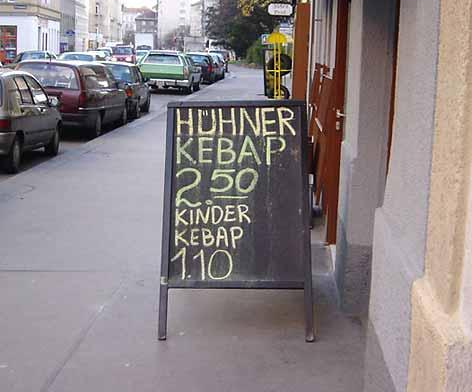
\includegraphics[scale=.55]{material/05Morph-Kebap}
%\end{figure}

\end{frame}


%%%%%%%%%%%%%%%%%%%%%%%%%%%%%%%%%%
%%%%%%%%%%%%%%%%%%%%%%%%%%%%%%%%%%
\subsubsubsection{Rektionskomposita}
%\frame{
%\frametitle{~}
%	\tableofcontents[currentsection]
%}


%%%%%%%%%%%%%%%%%%%%%%%%%%%%%%%%%%
\begin{frame}
\frametitle{Rektionskomposita}

\begin{itemize}
	\item Wichtige \textbf{Untergruppe} der Determinativkomposita:
	
	\eal \label{ex:Bsp1} 
        \ex die Linguisten tagen
        \ex die Tagung der Linguisten
        \ex Linguistentagung
	\zl
	
	\eal \label{ex:Bsp2} 
        \ex die Linguisten besteigen den Watzmann
        \ex die Besteigung des Watzmann
        \ex Watzmannbesteigung
	\zl
		 
\end{itemize}


\end{frame}


%%%%%%%%%%%%%%%%%%%%%%%%%%%%%%%%%%
\begin{frame}
\frametitle{Rektionskomposita}

\begin{itemize}
	\item \textbf{deverbale} Nomina (durch Derivation)
	
	\begin{itemize}
		\item[]
		\item tagen \ras Tagung
		\item[]
		\item Verb bestimmt mit wie vielen und mit welchen Argumenten es im Satz erscheint\\
                  (s. Rektion, Subkategorisierungsrahmen)
		
		\begin{itemize}
			\item[]
			\item Tagen in \ref{ex:Bsp1} + Subjekt
			\item[]
			\item besteigen in \ref{ex:Bsp2} + Subject + Objekt
			\item[]
			\item Beziehung zwischen Verb und seinen Argumenten auch innerhalb eines Kompositums
		\end{itemize}
	\end{itemize}
\end{itemize}


\end{frame}


%%%%%%%%%%%%%%%%%%%%%%%%%%%%%%%%%%
\begin{frame}
\frametitle{Rektionskomposita}

\begin{itemize}
	\item Rektionskompositum: \\
	die erste Konstituente in einem deverbalen Rektionskompositum realisiert ein Argument des der zweiten Konstituente zugrunde liegenden Verbs
	
	\begin{itemize}
		\item[]
		\item In \ref{ex:Bsp1}: \emph{Linguist(en)} \ras Subjekt von \emph{tagen}
		\item[]
		\item In \ref{ex:Bsp2}: Watzmann \ras Objekt von besteigen
	\end{itemize}
	
	\ea	 Auto$\cdot$fahrer (jemand fährt Auto), \\
		 Wetter$\cdot$beobachter (jemand beobachtet das Wetter), \\
		 Rotkehlchen$\cdot$gesang (das Rotkehlchen singt)
	\z
		 
\end{itemize}


\end{frame}


%%%%%%%%%%%%%%%%%%%%%%%%%%%%%%%%%%
\begin{frame}
\frametitle{Rektionskomposita}

\begin{itemize}
	\item Es gibt auch Rektionskomposita, in denen die zweite Konstituente ein nicht-deverbales Nomen oder ein Adjektiv ist, denn auch Nomina und Adjektive können Argumente nehmen:
	
	\ea Prüfungsangst (Angst vor der Prüfung), \\
		 Todessehnsucht (Sehnsucht nach dem Tod)
	\z
		 
	\ea staatstreu (dem Staat treu), \\
		 fälschungssicher (vor Fälschung sicher), \\
		 bleifrei (von Blei frei)
	\z
		 
\end{itemize}


\end{frame}


%%%%%%%%%%%%%%%%%%%%%%%%%%%%%%%%%%
\begin{frame}
\frametitle{Rektionskomposita}

\begin{itemize}
	\item \textbf{Rektionskompositum:} \\
	Kompositum, bei dem die \textbf{erste Konstituente ein Argument} (Subj., Akk.-Obj., Dat.-Obj., Gen.-Obj., Präp.-Obj., etc.) der zweiten Konstituente ist.
	\item Bei Nicht-Rektionskomposita besteht keine Argumentrelation.
\end{itemize}


\end{frame}


%%%%%%%%%%%%%%%%%%%%%%%%%%%%%%%%%%
%%%%%%%%%%%%%%%%%%%%%%%%%%%%%%%%%%
\subsubsubsection{Possessivkomposita}
%\frame{
%\frametitle{~}
%	\tableofcontents[currentsection]
%}


%%%%%%%%%%%%%%%%%%%%%%%%%%%%%%%%%%
\begin{frame}
\frametitle{Possessivkomposita}

\begin{itemize}
	\item Auch bei Possessivkomposita bestimmt die erste Konstituente die zweite näher.
	\item[]
	\item Das Kompositum bezieht sich aber auf \textbf{eine dritte Entität}, sie sind \textbf{exozentrisch}
	
	\ea \emph{Rot$\cdot$kehlchen} = Vogel, der ein rotes Kehlchen hat, nicht ein rotes Kehlchen ist
	\z
	
	\ea \emph{Rot$\cdot$käppchen} = Person, die eine rote Kappe hat (Märchenfigur), kein Käppchen
	\z
	
	\ea \emph{Lang$\cdot$finger} = Person, die lange Finger hat (= die stiehlt), kein Finger
	\z
	
\end{itemize}


\end{frame}


%%%%%%%%%%%%%%%%%%%%%%%%%%%%%%%%%%
%%%%%%%%%%%%%%%%%%%%%%%%%%%%%%%%%%
\subsubsubsection{Kopulativkomposita}
%\frame{
%\frametitle{~}
%	\tableofcontents[currentsection]
%}


%%%%%%%%%%%%%%%%%%%%%%%%%%%%%%%%%%
\begin{frame}
\frametitle{Kopulativkomposita}

\begin{itemize}
	\item Erste Konstituente \textbf{bestimmt} die zweite \textbf{nicht näher}
	\item[]
	\item Beide Konstituenten sind \textbf{gleichrangig}
	\item[]
	\item Auch aus mehr als zwei Konstituenten bestehend
	\item[]
	\item \textbf{Koordinierende} (= verknüpfende) Beziehung zwischen den Kompositionsgliedern
	\item[]
	\item Bedeutung des Kompositums ergibt sich \textbf{additiv}
	
	\eal 
	\ex süß$\cdot$sauer, nass$\cdot$kalt, rot$\cdot$grün, Fürst-Bischof
	\ex rot-rot-grün
	\zl
	
\end{itemize}


\end{frame}


%%%%%%%%%%%%%%%%%%%%%%%%%%%%%%%%%%
\begin{frame}
\frametitle{Kopulativkomposita}

\begin{itemize}
	\item Konstituenten in Kopulativkomposita \ras \textbf{gleiche Kategorie}
	\item Reihenfolge: prinzipiell frei, aber meistens \textbf{konventionalisiert}
	\item Anderes \textbf{Betonungsmuster} als Determinativkomposita
	
	\ea ein 'blau-'grünes 'Hemd - Kopulativ \\
		 ein 'blaugrünes 'Hemd - Determinativ
	\z
		 
	\item Während bei Determinativkomposita der Nichtkopf betont wird, werden bei Kopulativkomposita alle Konstituenten betont.
\end{itemize}


\end{frame}



%% \frame{
%% \frametitle{Kopulativkomposita}

%% Bei Kopulativkomposita gibt es keinen Kopf:
%% \ea
%% Fürstbischof = Fürst und Bischof gleichzeitig
%% \z

%% \pause
%% Unterschied zwischen \emph{grellweiß} und \emph{schwarz-weiß}.



%% }


\subsubsection{Derivation}


\frame{
\frametitle{Derivation}

\begin{itemize}
\item Komposition = Stamm + Stamm, Derivation = Stamm + Affix.
\pause
\item Beispiele für Regeln:

\medskip

\begin{tabular}{@{}ll@{}}
Beispiel & Regel\\
Erledigung, Beteiligung, Rechnung & N $\to$ V \suffix{ung}$_N$\\
lesbar, essbar, erklärbar & Adj $\to$ V \suffix{bar}$_{Adj}$\\
ungemütlich, unfreundlich, unschön & Adj $\to$ \prefix{un} Adj\\
Schönheit, Freiheit, Falschheit & N $\to$ Adj \suffix{heit}$_N$\\
\end{tabular}

\medskip

\pause
\item Kopf steht wieder rechts (Affixe haben Wortart)
\end{itemize}

}


\subsubsubsection{Selektion}

\frame{
\frametitle{Selektion}

Affixe gehen nicht mit beliebigem anderen Material zusammen,\\
sondern wählen sich ihren Partner aus.
\pause
\begin{itemize}
\item Wortart: \suffix{bar} verbindet sich nur mit Verben\\
      (nicht mit Adjektiven oder Nomina, bis auf unproduktive Ausnahmen)
\pause
\item Phonologische Restriktionen: \suffix{keit} verbindet sich nur mit mehrsilbigen Adjektiven, die
  auf eine unbetonte Silbe enden: \emph{Freundlichkeit}, \emph{Lesbarkeit}, \noword{Schönkeit},
  \noword{Freikeit}.
\pause
\item Bedeutung: \suffix{fach} verbindet sich nur mit Zahlen und Mengenangaben \emph{dreifach},
  \emph{mehrfach}, \noword{schönfach}, \noword{hausfach}
\pause
\item Morphologische Struktur: \gee verbindet sich nur mit morphologisch einfachen Verben
\emph{Gerenne}, \emph{Gehupe}, \noword{Geverkaufe}, \noword{Geanfange}
\end{itemize}


}

\subsubsubsection{Komplexe Verben}

\frame{
\frametitle{Komplexe Verben}

\begin{itemize}
\item Unterscheiden zwei Arten komplexer Verben: \\
Präfixverben (\emph{bestechen}, \emph{verlangen}, \emph{zersägen}) und Partikelverben
(\emph{ankaufen}, \emph{austrinken}, \emph{anlachen})
\begin{itemize}
\item Präfixverben verhalten sich wie Simplizia.
\item Partikelverben müssen in bestimmten syntaktischen bzw.\ morphologischen Umgebungen
  getrennt werden.
\eal
\ex dass Peter das Haus verkauft
\ex Peter verkauft das Haus.
\zl
\eal
\ex dass Peter das Glas austrinkt
\ex Peter trinkt das Glas aus.
\zl
\eal
\ex zersägt, zersägen
\ex ausgetrunken, auszutrinken
\zl

\end{itemize}


\end{itemize}

}


\subsubsection{Nichtkonkatenative Prozesse}

\subsubsubsection{Konversion}

\frame{
\frametitle{Nichtkonkatenative Prozesse: Konversion}


\begin{itemize}
\item Es gibt auch nichtkonkatenative Prozesse. Beispiel \blaubf{Konversion}
\item Wortart des Stammes wird geändert, ohne dass Material hinzugefügt würde.
\eal
\ex schlaf$_V$ $\to$ Schlaf$_N$
\ex grün$_{Adj}$ $\to$ grün$_{V}$
\ex braun$_{Adj}$ $\to$ bräun$_{V}$
\zl
\end{itemize}




}


\subsubsubsection{Kurzwortbildung}


\frame{
\frametitle{Kurzwortbildung und Kontamination}


\begin{itemize}
\item Kurzwortbildung
\eal
\ex Autobus $\to$ Bus
\ex Universität $\to$ Uni
\zl
\pause
\item Kontamination
\eal
\ex jein (jein = ja + nein)
\ex Teuro (teuer + Euro)
\zl


\end{itemize}





}


\subsection{Flexion}

\author{Stefan Müller (Anke Lüdeling)}

\frame[shrink=10]{
\frametitle{Flexion}

\begin{itemize}
\item Wortbildung beschäftigt sich mit Bildung neuer Lexeme.
\pause
\item Wortformen eines Lexems werden in verschiedenen Kontexten benötigt:
\begin{tabular}{@{}l@{~}l@{~}l@{~}l@{~}l@{}}
Klaus           & schmiert   & ein & belegtes & Brot.\\
Klaus           & schmierte  & ein & belegtes & Brot.\\
Klaus und Karin & schmierten & die & belegten & Brote.\\
Du              & schmierst  &     & belegte  & Brote.\\
\end{tabular}
\pause
\item Formen von \emph{schmieren} unterscheiden sich in Person, Numerus bzw.\ Tempus.
\pause
\item Formen von \emph{belegt} unterscheiden sich in Numerus und Stärke.
\pause
\item Formen von \emph{Brot} unterscheiden sich im Numerus.
\pause
\item Der Bereich, der sich mit diesen Variationen beschäftigt, heißt \alert{Flexion}.
\pause
\item Wie bei Derivation werden bei der Flexion Stämme mit einem oder mehreren Affixen kombiniert.
\pause
\item Art der Affixe hängt von Wortart ab.

\end{itemize}


}

\subsubsection{Wortarten}

\frame{
\frametitle{Wortarten}

\begin{itemize}
\item Wortarten sind Klassen von Wörtern mit ähnlichem Eigenschaften.
\pause
\item Klassische Wortarten (2. Jh. v. Chr.): Nomen, Verb, Partizip, Artikel, Pronomen, Präposition,
Adverb, Konjunktion
\pause
\item Beispiel für Definition:
\begin{quote}
Das Nomen ist ein kasusbildender Satzteil, welcher ein Ding, z.B. Stein, oder eine Handlung,
z.B. Erziehung, bezeichnet [\ldots].\\
Das Nomen hat fünf verschiedene Begleiterscheinungen:\\
Geschlecht, Art, Form, Zahl und Kasus.
\end{quote}
\pause
\item Vermischung verschiedener Kriterien aus Syntax, Semantik und Morphologie.

\pause
\item Unterscheidung zwischen flektierbaren und nichtflektierbaren Wortarten.
\end{itemize}

}


\frame{
\frametitle{Flektierbare und unflektierbare Wortarten}

\vfill
\begin{tabular}{|l|l|l|l|l|l|}\hline
\multicolumn{3}{|l|}{flektierbare Wortarten} & \multicolumn{3}{l|}{unflektierbare Wortarten}\\\hline
Name     & Abk. & Beispiele & Name         & Abk. & Beispiele\\\hline
Nomen    & N         & Tisch      & Präposition  & P         & auf, neben\\
         &           & Haus,Suppe &              &           & während\\\hline
%
Verb     & V         & koch, ess & Adverb       & Adv       & oft \\
         &           & schlaf    &              &           & gestern\\ \hline
%
Adjektiv & Adj       & schnell   & Konjunktion  & C         & dass,\\
         &           & blau      &              &           & weil,\\
         &           &           &              &           & und, oder\\\hline
%
Artikel  & D         & der, ein  & Interjektion & Int       & tja, pst, Hurra!\\\hline 
         &           &           & Partikel     & Part      & auf, an (mit Verb)\\
         &           &           &              &           & nur (drei Tage)\\\hline
\end{tabular}

\vfill

}

\subsubsubsection{Nicht flektierbare Wortarten}

\frame{
\frametitle{Nicht flektierbare Wortarten: Präpositionen}

\begin{itemize}


\item Nicht flektierbare können wir anhand ihrer syntaktischen Umgebung unterscheiden:


\alert{Präpositionen} werden mit einer Nominalgruppe kombiniert und bestimmen deren Kasus.
\eal
\ex \alert{auf} dem Sofa
\ex \alert{während} des Treffens
\zl

\pause
Präpositionalgruppen können sich auf Verben oder Nomina beziehen:
\eal
\ex die Zeitung auf dem Sofa
\ex Er schläft auf dem Sofa.
\zl

\end{itemize}

}

\frame{
\frametitle{Nicht flektierbare Wortarten: Konjunktionen}

\begin{itemize}
\item \alert{Konjunktionen} verbinden Teilsätze miteinander (\mex{1}a) oder ordnen Teilsätze einem Verb
unter (\mex{1}b):
\eal
\ex Er kommt später, \alert{weil} er noch arbeiten muss.
\ex Er glaubt, \alert{dass} er es noch schafft.
\zl

\pause
\item Auch in sogenannten Koordinationen kommen Konjunktionen vor:
\eal
\ex Er kennt \alert{und} liebt diese Schallplatte.
\ex Die Musik \alert{und} der Text ist von Frank Zappa.
\zl



\end{itemize}

}

\frame{
\frametitle{Nicht flektierbare Wortarten: Adverbien}

\alert{Adverbien} haben mehrere Funktionen.

\begin{itemize}
\item Sie modifizieren Verben (daher der Name):
\eal
\ex Max lacht \alert{oft}.
\ex Er kam \alert{gestern}.
\zl

\pause
\item Aber auch die Modifikation von Adjektiven ist möglich:
\eal
\ex das oft gelesene Buch
\ex das gestern gekaufte Buch
\zl

\pause
\item Vorsicht: Viele Adjektive können adverbial verwendet werden:
\ea
Er hat das Buch \alert{schnell} gelesen.
\z

\end{itemize}


}


\frame{
\frametitle{Nicht flektierbare Wortarten: Partikeln}

\begin{itemize}
\item Der Duden \citeyearpar{Duden2005} unterscheidet zwischen Adverbien und Partikeln.
\item \alert{Partikeln} sind wie Adverbien nicht flektierbar,\\
im Gegensatz zu Adverbien aber nicht voranstellbar:
\eal
\ex[]{
Max lacht oft.
}
\ex[]{
Oft lacht Max. (Adverb)
}
\zl
\eal
\ex[]{
Max hat sogar gelacht.
}
\ex[*]{
Sogar hat Max gelacht. (Partikel)
}
\zl
\end{itemize}

}

\frame{
\frametitle{Nicht flektierbare Wortarten: Interjektionen}

\begin{itemize}
\item  Interjektionen sind satzwertige Ausdrücke:

\begin{itemize}
\item Interjektionen im Gespräch:
\ea
Ja! Jawohl! Nein! Doch! Bitte! Danke! Servus!
              Adieu! Tschüs! Halt! Stopp! Marsch! Pst! He! Hallo!
\z

\pause
\item Interjektionen als Ausdruck von Empfindungen: 
\ea Hurra! Juchhe! Heißa! Ei!
              Bravo! Pfui! Ach! Oh! O weh! Ah! Hahaha! Potz! Hu! Hui! Iiiiii! Ätsch! Aha!
              Hm! Brrr!
\z
\pause
\item Tier- und Geräuschnachahmungen:  
\ea
Muh! Miau! Wauwau! Quak! Kikeriki!
              Knacks! Trara! Kling, klang! Piff, paff! Klipp, klapp! Plumps! Blabla!
\z
\end{itemize}
\end{itemize}

}




\subsubsubsection{Flektierbare Wortarten}

%\subsubsubsubsection{Nomina und Artikel}

\frame{
\frametitle{Nomina}


\begin{itemize}[<+->]
\item Deutsche Nomina haben ein Genus (masculin, feminin, neutrum).
\item Es gibt keine Beziehung zwischen Bedeutung und Genus (außer bei Personenbezeichnungen).
\item Genus ändert sich nicht in Abhängigkeit vom syntaktischen Kontext.\\
      Bezeichnung: \alert{inheränte Flexionskategorie}.
\item Abhängig vom Kontext Flexion nach Numerus (singular, Plural) und Kasus (Nominativ, Genitiv,
Dativ, Akkusativ).

\medskip


\begin{tabular}{|l|l|l|l|l|l|l|}\hline
          & \multicolumn{3}{l|}{Singular} & \multicolumn{3}{l|}{Plural}\\\hline
Nominativ & Tisch   & Suppe & Haus   & Tische  & Suppen & Häuser\\\hline
Genitiv   & Tisches & Suppe & Hauses & Tische  & Suppen & Häuser\\\hline
Dativ     & Tisch   & Suppe & Haus   & Tischen & Suppen & Häusern\\\hline
Akkusativ & Tisch   & Suppe & Haus   & Tische  & Suppen & Häuser\\\hline
\end{tabular}
\end{itemize}

}

\author{Stefan Müller}

\frame[shrink]{
\frametitle{Pronomina und Artikelwörter}


\begin{itemize}
\item Pronomina und Artikelwörter bilden eine Restkategorie.
\pause
\item Der Begriff \emph{Pronomen} kommt aus der Grammatik des Latein und steht
      traditionell sowohl für Artikel als auch für Wörter, die ganze Nominalgruppen ersetzen.
\pause
\item Das war sinnvoll, denn die Formen waren identisch.

Sie haben sich aber historisch auseinanderentwickelt.

\pause
\item Statt \emph{Pronomen} im obigen Sinn verwenden Grammatiken die stärker differenzierenden Begriffe \alert{Stellvertreter} und \alert{Begleiter}.

\pause
\item \alert{Artikel}/\alert{Determinator}: Element, das mit Nomen bzw.\ Adjektiven eine Nominalgruppe bildet
\pause
\item \alert{Pronomen}: Element, das für eine Nominalgruppe steht.

Zu den Pronomina werden auch die sogenannten Pronominaladverbien (\emph{darüber}, \emph{damit}, \ldots).

Diese stehen für Präpositionalgruppen (\emph{über dem Tisch}).
\end{itemize}

}

% \frame{
% \frametitle{Unterschied: definiter Artikel und Demonstrativpronomen}


% Die Formen des definiten Artikels und des Demonstrativpronomens sind meistens identisch,
% jedoch nicht immer:

% \medskip

% \begin{tabular}{|l|l|l|}\hline
% Kasus & Definiter Artikel & Demonstrativpronomen \\\hline
% Nom & der Mann   & der\\
% Gen & \alert{des} Mannes & \alert{dessen}\\
% Dat & dem Mann   & dem\\
% Akk & den Mann   & den\\\hline
% Nom & die Manner & die\\
% Gen & \alert{der} Männer & \alert{derer}\\
% Dat & \alert{den} Männern & \alert{denen}\\
% Akk & die Männer  & die\\\hline
% \end{tabular}


% }


\frame[shrink]{
\frametitle{Artikel/Determinator}

\begin{itemize}
\item Artikel stehen vor Nomina (oder Adjektiven) und bestimmen Definitheit:
\eal
\ex das/dieses/jenes Haus
\ex ein/kein Haus
\ex einige/mehrere Häuser
\zl

\pause
\item Klassisch: \alert{definiter Artikel} = \emph{der}, \emph{die}, \emph{das}
      \alert{indefiniter Artikel} = \emph{ein}

Duden-Grammatik nennt \emph{etwas}, \emph{nichts}, \emph{einige} \alert{indefinite Artikelwörter}
\eal
\ex etwas Farbe
\ex nichts Süßes
\ex einige Minuten
\ex alle Leute
\ex irgendwelche Kollegen
\zl

\end{itemize}

}

\author{Stefan Müller (Anke Lüdeling)}

\frame{
\frametitle{Artikel/Determinator: Flexionskategorien}

\begin{itemize}
\item Artikel haben dieselben Flexionskategorien wie Nomina.


\medskip


\begin{tabular}{|l|l|l|l|l|}\hline
          & \multicolumn{3}{l|}{Singular} & Plural\\\hline
Nominativ & der & die & das & die\\\hline
Genitiv   & des & der & des & der\\\hline
Dativ     & dem & der & dem & den\\\hline
Akkusativ & den & die & das & die\\\hline
\end{tabular}
\end{itemize}

}

\frame{
\frametitle{Synkretismus}

\begin{itemize}
\item Die Pluralformen sind für alle drei Genera identisch:

\medskip

\begin{tabular}{|l|l|l|l|l|}\hline
          & \multicolumn{3}{l|}{Singular} & Plural\\\hline
Nominativ & der & die & das & die\\\hline
Genitiv   & des & der & des & der\\\hline
Dativ     & dem & der & dem & den\\\hline
Akkusativ & den & die & das & die\\\hline
\end{tabular}

~

\pause
\item Auch im nominalen Paradigma fallen viele Formen zusammen.

Diesen Zusammenfall von Formen nennt man \alert{Synkretismus}.

\pause
\item Kasus lässt sich nicht eindeutig von der Form ablesen.

Kombination der Information von Artikel und Nomen hilft mitunter:
\eal
\ex der Tisch
\ex dem Tisch
\zl
\end{itemize}

}

\author{Stefan Müller}

\frame{
\frametitle{Synkretismus und Sexismus}

\begin{itemize}
\item Das hilft aber bei femininen Nomina nicht:
\ea
die Tochter (Nominativ oder Akkusativ)
\z
\pause

In Beispielen werden deshalb oft maskuline Nomina verwendet.

Kein Sexismus, sondern Vermeidung von Mehrdeutigkeit.

\pause
\item Meist hilft der Kontext, die Abfolge der Nominalgruppen im Satz oder die Prosodie:
\eal
\ex Den Vater liebt die Tochter nicht. Die Mutter liebt die Tochter.
\ex Die Mutter liebt den Sohn nicht. Die Mutter liebt die Tochter.
\zl

\end{itemize}

}


%{Pronomina}
\frame{
\frametitle{Pronomina -- I}

\begin{itemize}
\item \alert{Personalpronomen} (persönliche Fürwörter):\\
\emph{ich}, \emph{du}, \emph{er}, \emph{sie}, \emph{es}, \emph{wir}, \emph{ihr}, \emph{sie}

\pause
\item \alert{Possessivpronomen} (besitzanzeigende Fürwörter):\\
\emph{mein}, \emph{dein}, \emph{sein}, \emph{unser}, \emph{euer}, \emph{ihr}

\pause
\item \alert{Reflexivpronomen} (rückbezügliche Fürwörter):\\
\emph{mich}, \emph{dich}, \emph{sich}, \emph{uns}, \emph{euch}

\ea
Ich erhole \alert{mich}.
\z

\pause
\medskip
Reflexiv gebrauchtes Personalpronomen: auch Dativformen

\eal
\ex Ich wasche \alert{mich}.
\ex Ich wasche \alert{mir} den Rücken.
\zl

\pause
\alert{Reziprokpronomen} (wechselseitige Fürwörter): \emph{einander}

\end{itemize}


}


\frame{
\frametitle{Pronomina -- II}

\begin{itemize}

\item \alert{Demonstrativpronomen} (hinweisende Fürwörter):\\

    \emph{der}, \emph{dieser}, \emph{jener}, \emph{derjenige}, \emph{derselbe},\\
    \emph{die}, \emph{diese}, \emph{jene}, \emph{diejenige}, \emph{dieselbe},\\
    \emph{das}, \emph{dieses}, \emph{jenes}, \emph{dasjenige}, \emph{dasselbe}

\pause
\item \alert{Relativpronomen} (bezügliche Fürwörter):\\
\emph{der}, \emph{die}, \emph{das}, \emph{welcher}, \emph{welches}, \emph{welche},\\

\emph{wer}, \emph{was} (in freien Relativsätzen)

\pause
\item \alert{Interrogativpronomen} (fragende Fürwörter):\\
\emph{wer}, \emph{was}, \emph{welcher}

\pause
Frageadverbien auch hier einordnen? \emph{wofür}, \emph{womit}

\pause
\item \alert{Indefinitpronomen} (unbestimmte Fürwörter):\\
\emph{jemand}, \emph{alle}, \emph{einer}, \emph{keiner}, \emph{mancher}, \emph{man}, \emph{wer}, \emph{etwas}, \ldots

\end{itemize}


}

\author{Stefan Müller (Anke Lüdeling)}

\frame{
\frametitle{Adjektive: Flexionsklasse}

\begin{itemize}
\item Adjektive modifizieren Nomina (\mex{1}a) o.\ werden prädikativ verwendet (\mex{1}b):
\eal
\ex das rote Haus
\ex Das Haus ist rot.
\zl

\pause
\item Wie bei Nomina nach Kasus, Genus, Numerus unterschieden.
\pause
\item Zusätzlich Flexionsklasse: stark, schwach, gemischt:
\eal
\ex leckerer Auflauf, leckere Aufläufe\\ (ohne Artikel = stark)
\pause
\ex der leckere Auflauf, die leckeren Aufläufe\\ (definit = schwach)
\pause
\ex ein leckerer Auflauf, einige leckere Aufläufe\\ (ein/kein = gemischt)
\zl
\end{itemize}

}


\frame{
\frametitle{Adjektive: Grad}

\begin{itemize}
\item Flexion nach Grad:
\begin{itemize}
\item Positiv: \emph{lecker}
\item Komparativ: \emph{leckerer}
\item Superlativ: \emph{am leckersten}
\end{itemize}
\pause
\item Das ganze Paradigma unter \url{http://www.canoo.net/}.
\end{itemize}


}

\frame{
\frametitle{Verben}

\begin{itemize}
\item Verben unterteilen sich in Vollverben, Hilfsverben (Auxiliare) und Modalverben.
\pause
\item Vollverben teilen sich in schwache (regelmäßige) und starke (unregelmäßige) auf.\\
      Stark vs.\ schwach unterscheidet sich von den Klassen bei Adjektiven.
\pause
\item Vollverben und Hilfsverben flektieren nach Person, Numerus, Tempus, Modus und Genus Verbi.
\pause
\item Person und Nummerus sind für den syntaktischen Kontext wichtig (Kongruenz):

\medskip

~
\begin{tabular}{@{}lll@{}}
           & Singular  & Plural\\
1.\ Person & ich lache & wir lachen\\
2.\ Person & du lachst & ihr lacht\\
3.\ Person & er/sie/es lacht & sie lachen\\
\end{tabular}
\end{itemize}

}


\frame{
\frametitle{Verben: Tempus}

\begin{itemize}
\item Tempus, Modus und Genus Verbi fügen semantische Information hinzu.

\pause
\item Vereinfacht: Tempus sagt etwas darüber aus, wann die Handlung stattfindet.
\ea
Er lachte / lacht / wird lachen.
\z
\pause
\item Allerdings kann Präsens auch in Sätzen benutzt werden, die die Vergangenheit oder Zukunft beschreiben:
\eal
\ex Napoleon wird 1769 in Ajaccio auf der Insel Korsika geboren.
\ex Kommt er gestern in die Küche
\ex Ich bringe den Müll morgen runter.
\zl

\pause
\item Es gibt morphologisch einfache Formen und zusammengesetzte mit Hilfsverb + Partizip/Infinitiv.

\end{itemize}

}



\frame{
\frametitle{Flexionsparadigma: schwaches Verb, Aktiv, Indikativ}

\oneline{\begin{tabular}{|l|l|l|l|l|l|l|}\hline
Person \& & Präsens & Präteri- & Perfekt & Plusquam- & Futur I & Futur II\\
Numerus   &         & tum      &         & perfekt   &         &         \\\hline
%
1.\ Sg    & koche   & kochte   & habe    & hatte     & werde   & werde \\
          &         &          & gekocht & gekocht   & kochen  & gekocht haben\\\hline
%
2.\ Sg    & kochst  & kochtest & hast    & hattest   & wirst   & wirst \\
          &         &          & gekocht & gekocht   & kochen  & gekocht haben\\\hline
%
3.\ Sg    & kocht   & kochte   & hat     & hatte     & wird    & wird\\
          &         &          & gekocht & gekocht   & kochen  & gekocht haben\\\hline
%
1.\ Pl    & kochen  & kochten  & haben   & hatten    & werden & werden\\
          &         &          & gekocht & gekocht   & kochen & gekocht haben\\\hline
%
2.\ Pl    & kocht   & kochtet  & habt    & hattet    & werdet & werdet\\
          &         &          & gekocht & gekocht   & kochen & gekocht haben\\\hline
%
3.\ Pl    & kochen  & kochten  & haben   & hatten    & werden & werden\\
          &         &          & gekocht & gekocht   & kochen & gekocht haben\\\hline
\end{tabular}}


}

\frame{
\frametitlefit{Flexionsschema: schwache Verben, Präsens, Indikativ, Aktiv}


\vfill

\hfill
\begin{tabular}{|l|l|l|}\hline
Person \& & \multicolumn{2}{c|}{Präsens}\\
Numerus   &  \multicolumn{2}{c|}{} \\\hline
%           
1.\ Sg    &        & \suffix{e}\\\cline{1-1}\cline{3-3}
%           
2.\ Sg    &        & \suffix{st}\\\cline{1-1}\cline{3-3}
%           
3.\ Sg    &        & \suffix{t}\\\cline{1-1}\cline{3-3}
%           
1.\ Pl    & Stamm  & \suffix{en}\\\cline{1-1}\cline{3-3}
%           
2.\ Pl    &        & \suffix{t}\\\cline{1-1}\cline{3-3}
%           
3.\ Pl    &        & \suffix{en}\\\hline
\end{tabular}\hfill\hfill\mbox{}

\vfill

}

\frame{
\frametitle{Modus}


\begin{itemize}
\item Verbmodus: Indikativ, Konjunktiv I, Konjunktiv II
\pause
\item Bedeutung unscharf, kann aber wie folgt umrissen werden:
\begin{itemize}
\item Indikativ teilt Faktum mit
\ea
Max schläft. (Ich habe es selbst gesehen.)
\z
\pause
\item Konjunktiv I: Man hat von etwas gehört.
\ea
Barbara sagt, Max schlafe. (Ich glaube Barbara.)
\z
\pause
\item Konjunktiv II: Man hat von etwas gehört und zweifelt es an.
\ea
Barbara sagt, Max schliefe. (Ich glaube Barbara nicht.)
\z
\end{itemize}
\end{itemize}


}


\frame{
\frametitle{Genus Verbi}




\begin{itemize}
\item Genus Verbi: Aktiv und Passiv

\eal
\ex Er schlägt den Weltmeister.
\ex Der Weltmeister wird geschlagen.
\zl
\pause
\item Passiv = Unterdrückung des Subjekts (Agens im weiteren Sinne)
\pause
\item Die häufigste Form des Passivs wird mit dem Hilfsverb \emph{werden} gebildet.

\end{itemize}

}

\frame{
\frametitle{Andere Verbformen}


\eal
\ex geben (Infinitiv)
\pause
\ex gebend (Partizip Präsens)
\pause
\ex gegeben (Partizip Perfekt)
\pause
\ex gib (Imperativ Singular)
\pause
\ex gebt (Imperativ Plural)
\zl


}

\frame{
\frametitle{Modalverben und \emph{wissen}}


\begin{itemize}
\item Modalverben (\emph{dürfen}, \emph{können}, \emph{mögen}, \emph{müssen}, \emph{sollen}, \emph{wollen}),\\
      und damit gebildete Präfix- oder Partikelverben (\emph{bedürfen}, \emph{durchmüssen})\\
      und das Verb \emph{wissen} verhalten sich etwas anders.
\item Im Präsens verwenden sie die Präteritumsendungen der starken Verben.

~

\vfill


\hfill
\begin{tabular}{|l|l|l|l|l|}\hline
Person \& & \multicolumn{2}{c|}{Präteritum starke Verben} & \multicolumn{2}{c|}{Präsens Modalverben}\\
Numerus   &  \multicolumn{2}{c|}{} & \multicolumn{2}{c|}{} \\\hline
%           
1.\ Sg    &                  & $\varnothing$    && $\varnothing$    \\\cline{1-1}\cline{3-3}\cline{5-5}
%                                                                                    
2.\ Sg    & Präteritumsstam  & \suffix{st}      & Stamm & \suffix{st}      \\\cline{1-1}\cline{3-3}\cline{5-5}
%                                                                                    
3.\ Sg    & \emph{kam}       & $\varnothing$    & \emph{darf}/\emph{dürf}& $\varnothing$    \\\cline{1-1}\cline{3-3}\cline{5-5}
%                                                                                    
1.\ Pl    & \emph{schlief}   & \suffix{en}      & \emph{will}/\emph{woll} & \suffix{en}      \\\cline{1-1}\cline{3-3}\cline{5-5}
%                                                                                    
2.\ Pl    &                  & \suffix{t}       && \suffix{t}       \\\cline{1-1}\cline{3-3}\cline{5-5}
%                                                                                    
3.\ Pl    &                  & \suffix{en}      && \suffix{en}      \\\hline
\end{tabular}\hfill\hfill\mbox{}

\vfill

\end{itemize}

}

\subsubsubsection{Überblick}

\author{Stefan Müller (Peter Gallmann)}

\frame{
\frametitle{Überblick über die Wortarten (Peter Gallmann/Duden)}

\vfill

% used to work without tabular, I do not know why it needs tabular here. Maybe order of loading of packages
\centerfit{%
\begin{forest}
word tier, for tree={fit=rectangle}
[Wortart
       [flektierbar
          [nach Tempus [Verb] ]
          [nach Kasus 
            [festes Genus [Noun] ]
            [veränderbares Genus 
               [nicht komparierbar [\begin{tabular}{@{}c@{}}Artikelwort\\Pronomen\end{tabular} ] ]
               [komparierbar [Adjektiv] ] ] ] ]
       [nicht flektierbar [\begin{tabular}{@{}c@{}}Adverb\\Konjunktion\\Präposition\\Interjektion\end{tabular}] ] ]
\end{forest}
}

\vfill

}

\author{Stefan Müller (Anke Lüdeling)}

\subsubsection{Form und Funktion}

\frame{
\frametitle{Form und Funktion: Portmanteau-Morpheme}

\begin{itemize}
\item Wortbildung: Jedes Morphem hat eine Funktion/Bedeutungsbeitrag:
\eal
\ex Haus+tür
\ex Stör+ung
\zl

\pause
\item Flexion: Mitunter fallen mehrere Funktionen zusammen:
\eal
\ex ich lache -- lachte
\ex er lacht -- lachte
\zl
Steht das \suffix{t} für Präteritum, wie (\mex{0}a) nahelegt?

\pause
Steht das \suffix{e} für Präteritum, wie (\mex{0}b) nahelegt?

\pause
\item \suffix{te} ist ein kombiniertes Affix,\\
      das sowohl Tempus- als auch Kongruenzinformation enthält.

Solche Morpheme werden \alert{Portmanteau-Morpheme} oder \alert{Schachtelmorpheme} genannt.

\end{itemize}

}

\frame{
\frametitle{Form und Funktion: mehrfache Exponenten}

\begin{itemize}
\item Bei Portmanteau-Morphemen werden mehrere Funktionen von einem Morphem wahrgenommen.
\pause
\item Aber es gibt auch Fälle, in denen eine Funktion sich an mehreren Stellen manifestiert.

Beispiel: bestimmte Nomina im Deutschen, die mit Suffix und Umlautung den Plural bilden:
\ea
Mann -- Männer
\z
\end{itemize}

}



\frame{
\frametitle{Inhärente Flexion, regierte Flexion und Kongruenz}

\begin{itemize}
\item Flexion hilft bei der Bestimmung der Zusammengehörigkeit und Funktion von Elementen im Satz.
\item Können Flexionsinformation unterteilen in 
\begin{itemize}
\item inhärente Flexion, 
\item kontextabhängige Flexion,
\item regierte Flexion und 
\item Kongruenz

\end{itemize}

\end{itemize}

}

\frame{
\frametitle{Inhärente und kontextuelle Kategorien}

\begin{itemize}
\item Inhärente Flexionskategorien, \zb Genus bei Nomina oder Definitheit bei Artikeln: Diese
Informationen gehören zum Lexem, sie ändern sich nie. 

Sie können aber durchaus Auswirkungen auf andere Elemente in ihrer Umgebung haben.

\pause
\item Kontextuelle Kategorien, \zb Modus oder Tempus bei Verben. Solche Kategorien sind nicht durch
die Syntax vorgegeben, sondern durch das Informationsziel. 

\end{itemize}



}

\frame{
\frametitle{Regierte Flexion}

Regierte Kategorien, \zb Kasus bei nominalen Konstituenten in einer präpositionalen
Konstituente. 
\ea
in einem Korb
\z

Regierendes Element (\emph{in}) verlangt Dativ, steht aber nicht selbst im Dativ.

Durch Rektion wird Abhängigkeit aufgezeigt:\\
Alles, was von der Präposition abhängt, muss im Dativ stehen.
}

\frame{
\frametitle{Kongruenz}

Kongruenz: ein Element stimmt mit anderen Elementen in seiner Umgebung in einem oder mehreren
Merkmalen überein. 

\eal
\ex Max lacht.
\ex Max und Friederike lachen.
\zl
\eal
\ex ein gutes Ergebnis
\ex das gute Ergebnis
\ex des guten Ergebnisses
\zl

}

\subsection{Übung Derivation, Komposition, Flexion}

\frame{
\frametitle{Übung}

Analysieren Sie:
\eal
\ex Vorlesungsankündigung
\ex Straßenbahnhaltestelle
\ex Kinderschlafsack
\ex Kinderschreibtische
\zl

}

\frame{
\frametitle{Lösung: Vorlesungsankündigung}

\centerline{
\begin{forest}
sm edges
[N
  [N
    [N 
      [V 
        [Part [vor]]
        [V [les]]]
      [N-Aff [ung-s]]]
    [N [V [Part [an]]
          [V [kündig]]]
       [N-Aff [ung]]]]
  [Flex [$\varnothing$]]]
\end{forest}
}

\emph{kündigen}: mhd. für `mitteilen, künden'

}


\frame{
\frametitle{Lösung: Straßenbahnhaltestelle}

\centerline{%
\begin{forest}
sm edges
[N 
  [N
    [N
      [N [Straße-n]]
      [N [bahn]]]
    [N [V [halt-e]]
       [N [stelle]]]]
  [Flex [$\varnothing$]]]
\end{forest}}

}

\frame{
\frametitle{Lösung: Kinderschlafsack}

\centerline{%
\begin{forest}
sm edges
[N
  [N [N [kind-er]]
     [N
       [V [schlaf]]
       [N [sack]]]]
  [Flex [$\varnothing$]]]
\end{forest}
}

}

\frame{
\frametitle{Lösung: Kinderschreibtische}

\centerline{%
\begin{forest}
sm edges
[N
  [N [N [kind-er]]
     [N
       [V [schreib]]
       [N [tisch]]]]
  [Flex [e]]]
\end{forest}
}

}




%% -*- coding:utf-8 -*-

\subsection{Hausaufgaben}

\begin{frame}
	\frametitle{Hausaufgaben}

	
\begin{enumerate}
	 \item Kreuzen Sie die korrekten Aussagen an: %\hfill(0,5 Punkte pro Aussage)\\

\begin{itemize}
	\item[$\circ$] Die Graphemkette \emph{abarbeiten} ist ein einzelnes phonologisches Wort im Deutschen.
	\item[$\circ$] \emph{Morphologieeinführungsbuch} ist ein orthographisch-graphemisches Wort des Deutschen, sowie \emph{introductory morphology book} ein orthographisch-graphemisches Wort des Englischen ist.
	\item[$\circ$] Ein Morphem ist die kleinste bedeutungsunterscheidende Einheit in einem bestimmten Sprachsystem.
	\item[$\circ$] \ab{Brot} und \ab{Bröt} sind Allomorphe eines einzelnen Morphems.
\end{itemize}

	\item Erklären Sie das Prinzip der Rechtsköpfigkeit in der Morphologie des Deutschen. Verwenden Sie bei Ihrer Erklärung die unten angegebenen Beispiele.%\hfill(4 Punkte)\\

\eal
\ex lichtblau, Blaulicht
\ex die Fotowelt, das Weltfoto
\ex der Bücherrücken/die Bücherrücken, das Rückenbuch/die Rückenbücher
\zl
\end{enumerate}

\end{frame}



\begin{frame}
\frametitle{Hausaufgaben}
\begin{itemize}
	\item[3.] Geben Sie Argumente für oder gegen die Behandlung von \emph{ver-} in den folgenden Wörtern als Morphem an. Wenn es sich um ein Morphem handelt, ist das immer das gleiche Morphem? %(4 Punkte)

	\eal
	\ex \emph{Ver}zweiflung
	\ex \emph{Ver}s
	\ex \emph{ver}kaufen
	\ex \emph{ver}schreiben
	\ex \emph{ver}fahren
	\zl

\end{itemize}
\end{frame}



\begin{frame}
	\frametitle{Hausaufgaben}
	
\begin{itemize}
\item[4.] Ordnen Sie die Wortbildungsprozesse links den passenden Beispielen rechts zu (dazu müssen Sie nur den entsprechenden Buchstaben neben das passende Beispiel schreiben). %(0,5 Punkte pro Aussage)
\end{itemize}

\begin{table}[h!]
	\begin{minipage}{0.4\linewidth}
		\centering
		\begin{tabular}{l|p{0.1\textwidth}|}
			Determinativkompositum & (A)\\
			\hline
			Konversion & (B)\\
			\hline
			Zirkumfigierung (Derivation) & (C)\\
			\hline
			Rektionskompositum & (D)\\
			\hline
			Possessivkompositum & (E)\\
		\end{tabular}
		
	\end{minipage}\hfill%
	\begin{minipage}{0.4\linewidth}
		\centering
		\begin{tabular}{|p{0.1\textwidth}|r}
			& \emph{Gerede} \\
			\hline
			& \emph{Milchgesicht}\\
			\hline
			& \emph{Lauf} \\
			\hline
			& \emph{Kettenraucher}  \\
			\hline
			& \emph{Klausurbesprechung}  \\
		\end{tabular}
	\end{minipage}
\end{table}
\end{frame}



\begin{frame}
	\frametitle{Hausaufgaben}
\begin{itemize}
\item[5.] Warum sind die Wörter unter (i.) grammatisch und die unter (ii.) ungrammatisch? %(4 Punkte)
	\eal
	\ex kaufbar, trinkbar
	\ex *fensterbar, *helfbar, *schönbar
	\zl

      \item [6.] Sind die folgenden Verben Präfixverben oder Partikelverben? Begründen Sie Ihre Entscheidungen. %(3 Punkte)

	\eal
	\ex auskennen
	\ex erkennen
	\ex aberkennen
	\zl

\item [7.] Geben Sie für das folgende Wort eine morphologische Konstituentenstruktur (inklusive Konstituentenkategorien (N, N\textsuperscript{af}, V, V\textsuperscript{af}, \dots)) an, und bestimmen Sie für jeden Knoten den Wortbildungstyp. %(6,5 Punkte)

	\ea
	Wahlkampfberaterinnen
	\z

\end{itemize}

\end{frame}



\begin{frame}
	\frametitle{Hausaufgaben}
	
\begin{itemize}

\item [8.] Paraphrasieren Sie das folgende komplexe Wort so, dass es der angegebenen Struktur entspricht (auch wenn Sie selbst eine andere Struktur plausibler finden sollten). %(2 Punkte)

\begin{forest}sn edges,
	[N
	[N[N[Reserve]]
	[N[V[lehr]][N\textsuperscript{af}[-er]]]]
	[N[zimmer]]
	]
\end{forest}

\end{itemize}

\end{frame}


\begin{frame}
	\frametitle{Hausaufgaben}
	
\begin{itemize}

\item [9.] Geben Sie für die folgende Wortform die Flexionskategorien an, nach denen sie flektiert ist.\\
%\hfill(3 Punkte)\\
	\ea
	bestehe
	\z

\end{itemize}

\end{frame}

%%%%%%%%%%%%%%%%%%%%%%%%%%%%%%%%%%%%%%%%%%%%%%%%%%%%%%%%%%%%%%
%%%%%%%%%%%%%%%%%%%%%%%%%%%%%%%%%%%%%%%%%%%%%%%%%%%%%%%%%%%%%
\subsection{Lösungen}
%%%%%%%%%%%%%%%%%%%%%%%%%%%%%%%%%%%%%%%%%%%%%%%%%%%%%%%%%%%%%%
%%%%%%%%%%%%%%%%%%%%%%%%%%%%%%%%%%%%%%%%%%%%%%%%%%%%%%%%%%%%%
\begin{frame}
	\frametitle{Lösungen}

\begin{enumerate}
	\item Kreuzen Sie die korrekten Aussagen an: %\hfill(0,5 Punkte pro Aussage)\\
	
	\begin{itemize}
	\item[$\circ$] Die Graphemkette abarbeiten ist ein einzelnes phonologisches Wort im Deutschen.
	\item[$\circ$] \emph{Morphologieeinführungsbuch} ist ein orthographisch-graphemisches Wort des Deutschen, sowie \emph{introductory morphology book} ein orthographisch-graphemisches Wort des Englischen ist.
	\item[$\circ$] Ein Morphem ist die kleinste bedeutungsunterscheidende Einheit in einem bestimmten Sprachsystem.
	\textcolor{red}{\item[$\checkmark$] \ab{Brot} und \ab{Bröt} sind Allomorphe eines einzelnen Morphems.}
\end{itemize}
	
	\item Erklären Sie das Prinzip der Rechtsköpfigkeit in der Morphologie des Deutschen. Verwenden Sie bei Ihrer Erklärung die unten angegebenen Beispiele.%\hfill(4 Punkte)\\
	
		\eal
			\ex lichtblau, Blaulicht \ras Wortart
			\ex die Fotowelt, das Weltfoto \ras Genus und Semantik
			\ex der Bücherrücken/die Bücherrücken, das Rückenbuch/die Rückenbücher \ras Pluralflexion
		\zl		
\end{enumerate}

\end{frame}

%%%%%%%%%%%%%%%%%%%%%%%%%%%%%%%%%%%%%%%%%%%%%%%%%%%%%%%%%%%%

\begin{frame}
\frametitle{Lösungen}
\begin{itemize}
	\item[3.] Geben Sie Argumente für oder gegen die Behandlung von \emph{ver-} in den folgenden Wörtern als Morphem an. Wenn es sich um ein Morphem handelt, ist das immer das gleiche Morphem? %(4 Punkte)
	
	\eal \label{ver}
	\ex\label{vera}  \emph{Ver}zweiflung
	\ex\label{verb} \emph{Ver}s
	\ex \label{verc} \emph{ver}kaufen
	\ex\label{verd}  \emph{ver}schreiben
	\ex\label{vere} \emph{ver}fahren
	\zl
	
	\textcolor{red}{
		Morphem: Kleinste bedeutungstragende Einheit im Sprachsystem.	
		\begin{itemize}
			\item[] \gqq{ver} in (\ref{verb})  \ras kein Morphem, sondern Bestandteil des Stammes.
			\item[] \gqq{ver} in (\ref{ver}a,c,d,e) \ras Morpheme, aber unterschiedliche Morpheme, weil sie unterschiedliche Bedeutungen tragen
			\item[] \gqq{ver} in (\ref{ver}d,e) trägt die Bedeutung \gq{X falsch machen} (d.h. \gq{falsch schreiben/fahren})
			\item[] \gqq{ver} in (\ref{verc}) kehrt die Bedeutung von X um (kaufen \ras verkaufen)
			\item[] \gqq{ver} in (\ref{vera}) trägt eine intensivierende(?) Bedeutung
		\end{itemize}
	}
\end{itemize}
\end{frame}

%%%%%%%%%%%%%%%%%%%%%%%%%%%%%%%%%%%%%%%%%%%%%%%%%%%%%%%%%%%%

\begin{frame}
\frametitle{Lösungen}

\begin{itemize}
	\item[4.] Ordnen Sie die Wortbildungsprozesse links den passenden Beispielen rechts zu (dazu müssen Sie nur den entsprechenden Buchstaben neben das passende Beispiel schreiben). %(0,5 Punkte pro Aussage)
\end{itemize}

	\begin{table}[h!]
	\begin{minipage}{0.4\linewidth}
		\centering
		\begin{tabular}{|l|p{0.1\textwidth}|}
			\hline 
			Determinativkompositum & (A)\\
			\hline
			Konversion & (B)\\
			\hline
			Zirkumfigierung (Derivation) & (C)\\
			\hline
			Rektionskompositum & (D)\\
			\hline
			Possessivkompositum & (E)\\
			\hline 
		\end{tabular}
		
	\end{minipage}\hfill%
	\begin{minipage}{0.4\linewidth}
		\centering
		\begin{tabular}{|p{0.1\textwidth}|r|}
			\hline 
			\textcolor{red}{C} & \emph{Gerede} \\
			\hline
			\textcolor{red}{E} & \emph{Milchgesicht}\\
			\hline
			\textcolor{red}{B} & \emph{Lauf} \\
			\hline
			\textcolor{red}{A} & \emph{Kettenraucher}  \\
			\hline
			\textcolor{red}{D} & \emph{Klausurbesprechung}  \\
			\hline 
		\end{tabular}
	\end{minipage}
\end{table}
\end{frame}

%%%%%%%%%%%%%%%%%%%%%%%%%%%%%%%%%%%%%%%%%%%%%%%%%%%%%%%%%%%

\begin{frame}
\frametitle{Lösungen}
\begin{itemize}
	\item[5.] Warum sind die Wörter unter (\ref{kauf}) grammatisch und die unter (\ref{fenster}) ungrammatisch? %(4 Punkte)
	\eal
	\ex\label{kauf} kaufbar, trinkbar
	\ex\label{fenster} *fensterbar, *helfbar, *schönbar
	\zl
	
	\textcolor{red}{
		Das Suffix \gqq{-bar} hat die folgenden Beschränkungen bzgl. der Basis X, mit der es sich verbindet:
		\begin{itemize}
			\item[] X muss ein Verb sein (nicht Nomen oder Adjektiv)
			\item[] X muss transitiv sein (nicht wie \gqq{helfen})
		\end{itemize}
	}

	\item [6.] Sind die folgenden Verben Präfixverben oder Partikelverben? Begründen Sie Ihre Entscheidungen. %(3 Punkte)
	
	\eal
	\ex auskennen
	\ex erkennen
	\ex aberkennen
	\zl
	
	\textcolor{red}{
		Partikelverb: 1) morphologisch trennbar (\emph{aus-ge-kannt}, \emph{ab-zu-erkennen}), 2) syntaktisch trennbar (\gqq{Peter \emph{kennt} sich \emph{aus}}, \gqq{Die Frau \emph{erkennt} die Urkunde \emph{ab}}) und 3) die Partikel trägt die Hauptbetonung (\emph{AUSkennen} und \emph{ABerkennen}).
		Präfixverb: weder morphologisch noch syntaktisch trennbar (*\emph{ergekannt}, \gqq{*\emph{Peter kannte ihn er}}), Hauptbetonung liegt auf der Basis (\emph{erKENnen}).\\
		\bigskip
		EXTRA: \gqq{aberkennen} ist ein Partikelverb, welches aus einem Präfixverb und einer Partikel besteht (ab+erkennen).\\
	}
\end{itemize}

\end{frame}

%%%%%%%%%%%%%%%%%%%%%%%%%%%%%%%%%%%%%%%%%%%%%%%%%%%%%%%%%%%

\begin{frame}
	\frametitle{Lösungen}
	\item [7.] Geben Sie für das folgende Wort eine morphologische Konstituentenstruktur (inklusive Konstituentenkategorien (N, N\textsuperscript{af}, V, V\textsuperscript{af}, \dots)) an, und bestimmen Sie für jeden Knoten den Wortbildungstyp. %(6,5 Punkte)

\ea
Wahlkampfberaterinnen
\z

\textcolor{red}{
	%	\begin{figure}[h]
	\begin{forest} MyP edges,
		[N, name=N1
		[N, name=N2
		[N, name=N3
		[N, name=N4
		[N, name=N6 [V[wahl/wähl]]]
		[N, name=N7 [V[kampf/kämpf]]]]
		[N, name=N5[V, name=V1	[V\textsubscript{af}[be-]]
		[V[rat]]]
		[N\textsuperscript{af}[-er]]]]
		[N\textsuperscript{af}[-in]]]
		[Fl[-nen]]]	
		{
			\draw[<-, red] (N1.west)--++(-10em,0pt)
			node[anchor=east,align=center]{Flexion (KEIN Wortbildungsporzess)};
			\draw[<-, red] (N2.west)--++(-12em,0pt)
			node[anchor=east,align=center]{Derivation (Movierung)};
			\draw[<-, red] (N3.west)--++(-8em,0pt)
			node[anchor=east,align=center]{Determinativkompositum};
			\draw[<-, red] (N4.west)--++(-3em,0pt)
			node[anchor=east,align=center]{Determinativkompositum};
			\draw[<-, red] (N5.west)--++(-2em,0pt)
			node[anchor=east,align=center]{Derivation};
			\draw[<-, red] (N6.west)--++(-2em,0pt)
			node[anchor=east,align=center]{Implizite Derivation};
			\draw[<-, red] (N7.east)--++(2.5em,0pt)--++(0em,-18ex)%--++(2em,0pt)
			node[anchor=north,align=center]{Implizite Derivation};
			\draw[<-, red] (V1.east)--++(1.5em,0pt)--++(0em,-14ex)--++(2em,0pt)
			node[anchor=west,align=center]{Derivation};
		}	
	\end{forest}	
	%	\end{figure}
}
\end{frame}


%%%%%%%%%%%%%%%%%%%%%%%%%%%%%%%%%%%%%%%%%%%%%%%%%%%%%%%%%%%

\begin{frame}
\frametitle{Lösungen}

\begin{itemize}
	
	\item [8.] Paraphrasieren Sie das folgende komplexe Wort so, dass es der angegebenen Struktur entspricht (auch wenn Sie selbst eine andere Struktur plausibler finden sollten). %(2 Punkte)
	
	\begin{forest}sn edges,
		[N
		[N[N[Reserve]]
		[N[V[lehr]][N\textsuperscript{af}[-er]]]]
		[N[zimmer]]
		]
	\end{forest}
	
	\item[] \textcolor{red}{
		Ein Zimmer für Reservelehrer
	}
\end{itemize}

\end{frame}

%%%%%%%%%%%%%%%%%%%%%%%%%%%%%%%%%%%%%%%%%%%%%%%%%%%%%%%%%%%

\begin{frame}
\frametitle{Lösungen}

\begin{itemize}

\item [9.] Geben Sie für die folgende Wortform die Flexionskategorien an, nach denen sie flektiert ist.\\
%\hfill(3 Punkte)\\
\ea
bestehe
\z

\item [] \textcolor{red}{
	1. \ras 1.P. / Sg. / Präsens / Indikativ / Aktiv\\
	2. \ras 1.P. / Sg. / Präsens / Konjunktiv I / Aktiv\\
	3. \ras 3.P. / Sg. / Präsens / Konjunktiv I / Aktiv\\
	4. \ras 2.P. / Sg. / Präsens / Imperativ / Aktiv\\
}
\end{itemize}

\end{frame}



%% -*- coding:utf-8 -*-

%%%%%%%%%%%%%%%%%%%%%%%%%%%%%%%%%%%%%%%%%%%%%%%%%%%%%%%%%


\def\insertsectionhead{\refname}
\def\insertsubsectionhead{}

\huberlinjustbarfootline


\ifpdf
\else
\ifxetex
\else
\let\url=\burl
\fi
\fi
\begin{multicols}{2}
{\tiny
%\beamertemplatearticlebibitems

\bibliography{gkbib,bib-abbr,biblio}
\bibliographystyle{unified}
}
\end{multicols}





%% \section{Literatur}
%% \begin{frame}[allowframebreaks]
%% \frametitle{Literatur}
%% 	\footnotesize

%% \bibliographystyle{unified}

%% 	%German
%% %	\bibliographystyle{deChicagoMyP}

%% %	%English
%% %	\bibliographystyle{chicago} 

%% 	\bibliography{gkbib,bib-abbr,biblio}
	
%% \end{frame}


\end{document}
